\section{Основні алгоритми}
\subsection{Віднімання фону}
Віднімання фону дуже поширений алгоритм, який використовується у ситуаціях, коли відомо, що камера відносно нерухома. Завдяки йому можна достатньо просто виділити фон із зображення, а значить і передній план чи просто об'єкти, які динамічно рухаються на відео.

Часто використовується для обробки відео з дорожніх відеорегістраторів чи IP камер, які розташовані у людних місцях. Відніманням фону можна миттево отримати усі рухомі об'єкти на відео - машини, пішоходи тощо. Також є певні модифікації цього алгоритму для виділення навіть об'єктів, що не рухаються певний час, проте вони більш пристосовані під окремі задачі.

\subsubsection{Математичні основи}
\begin{equation}
\label{eq:background_substraction}
P[F(t)] = P[I(t)] - P[B]
\end{equation}
де $P[B]$ - зображення фону, $P[I(t)]$ - поточне зображення, $P[F(t)]$ - різниця між поточним зображенням та фоном.

За умови незмінності фону можна працювати з формулою (\ref{eq:background_substraction}).

Для відслідковування рухів динамічних об'єктів також використовується рівняння:
\begin{equation}
\label{eq:frames_difference}
\|P[F(t)] - P[F(t+1)]\| > Treshold
\end{equation}
де $Treshold$ - деяка задана порогова величина.

\begin{figure}[H]
	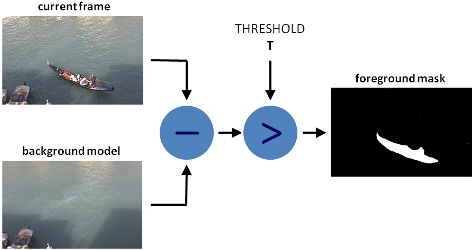
\includegraphics[width=0.9\linewidth]{theory/img/background_substraction}
	\caption{Ілюстрація роботи простого алгоритма віднімання фону}
\end{figure}

Тобто маючи попередньо зображення фону можна отримати передній план зображення просто віднявши від поточного зображення поелементно зображення фону.

Також існують підходи, за яких зберігається не фонове зображення, а історія N останніх зображень. Такі алгоритми називають змішаними.

Нехай у деякий момент $t = t^{*}$ у пам'яті зберігається історія $N$ останніх фреймів відео $P[I(t^{*} - 1)], ... , P[I(t^{*} - N)]$, $\lambda_{1}, ... , \lambda_{N} : \sum_{i = 1}^{N} \lambda_{i} = 1$ - ваги, тоді фонове зображення може бути виражене як:
\begin{equation}
	P[F(t^{*})] = \sum_{ i = 1}^{N} \lambda_{i} * P[I(t^{*} - i)]
	\label{eq:background_approximation}
\end{equation}

Від вибору $\lambda_{i}$ залежить значимість віддалених у часі фреймів у фоновому зображенні.Якщо взяти їх усіх рівними $\frac{1}{N}$, то такий алгоритм називають змішаною моделю середнього значення віднімання фону. 

Виділення переднього фону можна записати як:
\begin{equation}
Foreground[I(t^{*})] = | P[F(t^{*})] - P[I(t^{*})] | > Threshold
\label{eq:foreground_extraction}
\end{equation}
$| P[F(t^{*})] - P[I(t^{*})] | > Threshold$ у формулі \ref{eq:foreground_extraction} слід розуміти як поелементна різниця матриць і поелементне порівняння цієї різниці з певною пороговою величиною. Тобто на виході отримане бінарне зображення - матриця з 0 та 1.

\subsubsection{Особливості реалізації}

У роботі використовується змішана гаусівська модель віднімання фону, що описана у \cite{MOG1} та \cite{MOG2}. Така модель краща за звичайну модель середнього значення через те, що чим більше віддалена від поточного зображення фрейм, тим менша його значимість на данний момент. Також гаусівский розподіл дуже добре себе показує у багатьох ситуаціях. Звісно можна вибрати коефіцієнти згідно з рядом фібоначі, проте гаусівський розподіл показує кращі результати.

\subsection{Байесовський класифікатор}
\jointitles
\subsubsection{Теоретичні засади}

Цей підхід зустрічається у літературі дуже часто і основна формула, що описує модель, на перший погляд незрозуміла:
\begin{equation}
\label{eq:bayesian_classifier}
P(s|c) = \frac{P(c|s) * P(s)}{P(c)}
\end{equation}

Це звичайний запис теореми Байеса для знаходження апостеріорних ймовірностей.

$P(s|c)$ - ймовірність того, що піксель належить до множини кольорів шуканого об'єкта за умови що піксель має колір $c$. $P(s|c)$ в свою чергу має обернене формулювання - ймовірність того, що піксель приймає значення $c$ за умови що він належить до множини кольорів об'єкта.
$P(s)$ - ймовірність того, що піксель належить до множини кольорів об'єкта. $P(c)$ - загальна ймовірність того, що піксель має колір $c$.

\subsubsection{Пристосування до задачі розпізнавання кольорів об'єкта}

З формули \ref{eq:bayesian_classifier} не зовсім зрозуміло як взягалі шукати 3 ймовірності, що присутні у правій частині рівності.

Основне припущення цього підходу - кольори окремих пікселей на рображенні незалежні один від одного. За такого припущення можна сказати, що $P(s)/P(c)$ - деяка загальна константа якою можна знехтувати поставивши її рівною 1, а $P(c|s) = m/n$, де $m$ - кількість пікселів кольору $c$, що належать об'єкту, $n$ - загальна кількість пікселів, що належала об'єкту.

\subsubsection{Корекція моделі}
Приймаючи до уваги, що в задачі розпізнавання людської руки на відео класифікатор використовується лише для 2 із 3 компонент колірного простору, в якому є виділення люмінантної складової в окрему компоненту, то результатом навчання класифікатора слід очікувати деяку матрицю ймовірностей.

Основною ідеєю корекції моделі є те, що навчання могло проводитись не зовсім якісно і тому деякі ймовірності можуть бути лише поодинокими шумами. Матрицю ймовірностей можна розцінювати як деяке зображення та його обробку можна також розцінювати як обробку специфічного зображення.

Перший підхід до обробки матриці ймовірностей має прив'язку лише до чи нульова певна ймовірність.
\begin{equation}
	A[i,j] = ( P[i,j] > 0 )
\end{equation}
де $P$ - матриця ймовірностей.

Матриця $A$ складається лише з 0 та 1. Наступним кроком є застосування згортки з ядром, що складається лише з 1 та має форму круга з радіусом $R$. Це ядро ненормоване, тобто сумма усіх його елементів не рівна 1. Таким чином буде отримана матриця $N$, що її $(i,j)$ елемент приймає значення кількості його ненульових сусідів у радіусі $R$ навколо нього. Тобто побудована матриця $N$ на позиції $(i,j)$ містить число ненульових ймовірностей матриці $P$ у крузі з центром в $(i,j)$ та радіуса $R$. Заключним кроком є занулювання усіх ймовірностей, що мають недостатню кількість ненульових сусідів у відсотках від площі круга згорткового ядра. Таким чином після цієї процедури вигляд матриці ймовірностей більш заокруглений та не містить поодиноких ймовірностей.

Другий підхід приймає до уваги не тільки факт того, що ймовірність ненульова, а і її значення.
Відрізняється він тим, що у якості згорткового ядра береться гаусівське ядро, яке нормоване і тому результат згортки також буде знаходитись у межах $[0,1]$. Усі ймовірності, що менші за задане значення зануляються. Тобто результат згортки зберігається в окремій матриці
\subsubsection{Удосконалення процесу навчання класифікатора}

Оскільки процес навчання класифікатора доволі тривалий через те, що треба вручну обробляти велику кількість фотографій, то є сенс подумати над іншими можливими шляхами навчання.

У цій роботі використовується камера Intel Realsense F200, яка окрім кольорової камери має ще і сенсор глибини. Завдяки вбудованій у драйвер можливості отримувати синхронізовану карту глибини зображення є спосіб удосконалити та кардинально пришвидшити навчання класифікатора.

Карта глибини - матриця з цілими типу uint16 ( 16 бітне ціле беззнакове число ). 0 використовується для позначення неможливості визначити відстань.

Таким чином можна фільтрувати колірне зображення за відстанню та встановити межу 0.5м і усі пікселі, відстані до яких більша за встановлену границю, будуть мати чорний колір, який використовується для позначення пікселя, який не бере участь у навчанні.

\subsection{Обробка відеопотоку камери глибини}
Завдяки камері Intel Realsense F200 є можливість працювати з картами глибини зображення, проте для локалізації руки та подальшого аналізу жестів в цьому випадку дані про кольори насправді непотрібні. Вимикання колірного відеопотоку значно збільшує швидкість отримання зображення оскільки не виконується синхронізація двох відеопотоків, яка у драйвері навіть не оптимізована.

Обробка карт глибини ідентична до того, що вище було зазначено для кольорових зображень:
\begin{enumerate}
	\item Erode, dilate - для стабілізації геометричних контурів об'єктів;
	\item Розмиття - видалення шумів оскільки інфрачервоний сенсор цієї камери працює не зовсім стабільно та часто можна помітити випадкові шуми.
\end{enumerate}

Далі у загальному випадку за допомоги SimpleBlobDetector з бібліотеки opencv можна отримати усі blob елементи зображення та провести фільтрацію по певним параметрам - площа, кількість геометричних дефектів контура об'єкта тощо.